\documentclass[12pt,a4paper]{article}

% --- Packages essentiels ---
\usepackage[T1]{fontenc}
\usepackage[french]{babel}
\usepackage{amsmath, amssymb}
\usepackage{geometry}
\usepackage{graphicx}
\usepackage{tikz}
\usetikzlibrary{calc}
\usepackage{hyperref}
\usepackage{setspace}
\usepackage{xcolor}

% Gris pâle pour les blocs de code
\definecolor{lightgray}{RGB}{245,245,245}

% Minted settings
\usepackage{minted}
\setminted{
    fontsize=\small,
    breaklines=true,
    bgcolor=lightgray
}
% --- Minted for Isabelle/HOL code ---
\usepackage{minted}
\usemintedstyle{friendly}

% Required for minted
% (Ton workflow latexmk utilise déjà -shell-escape)

\setminted{fontsize=\small, breaklines=true}

\geometry{margin=1in}

% --- Hyperliens ---
\hypersetup{
    colorlinks=true,
    linkcolor=blue,
    urlcolor=blue,
    pdftitle={Postulat du Squaring},
    pdfauthor={Philippe Thomas Savard}
}

% Pas de numérotation sur la page titre
\pagenumbering{gobble}

\begin{document}



% --- Page titre ---
\begin{titlepage}
    \centering
    \vspace*{2cm}

    {\Huge \textbf{L'univers est au carré}}\\[0.5cm]
    {\Large \textbf{Chapitre : Le Postulat du Squaring}}\\[2cm]

    {\Large Auteur : \textbf{Philippe Thomas Savard}}\\[0.3cm]
    {\large Lévis, Chaudière-Appalaches, Canada}\\[0.3cm]
    {\large Treize mars deux mille vingt-six}\\[2cm]

    \vfill
\end{titlepage}

\clearpage
\pagenumbering{arabic}

\tableofcontents
\clearpage

% --- Message d'auteur ---
\begin{center}
\begin{minipage}{0.85\textwidth}
\small
\section*{Note de l’auteur}
\addcontentsline{toc}{section}{Note de l’auteur}

L’auteur de ce document n’a aucune formation académique reconnue. 
Il est ouvrier, et il a conçu ce travail sans financement, sans soutien institutionnel et sans aucun intérêt de quelque nature que ce soit. 
Ce document est rédigé et partagé librement, avec une pleine conscience et une lucidité entière.

Les sujets abordés relèvent des mathématiques et de la géométrie. 
Ils ont été explorés et développés par pur plaisir intellectuel, dans un esprit de curiosité, de rigueur personnelle et de liberté créative.
\end{minipage}
\end{center}

\vspace{1cm}

% --- Figure : Rectangle au carré ---
\begin{figure}[h!]
\centering
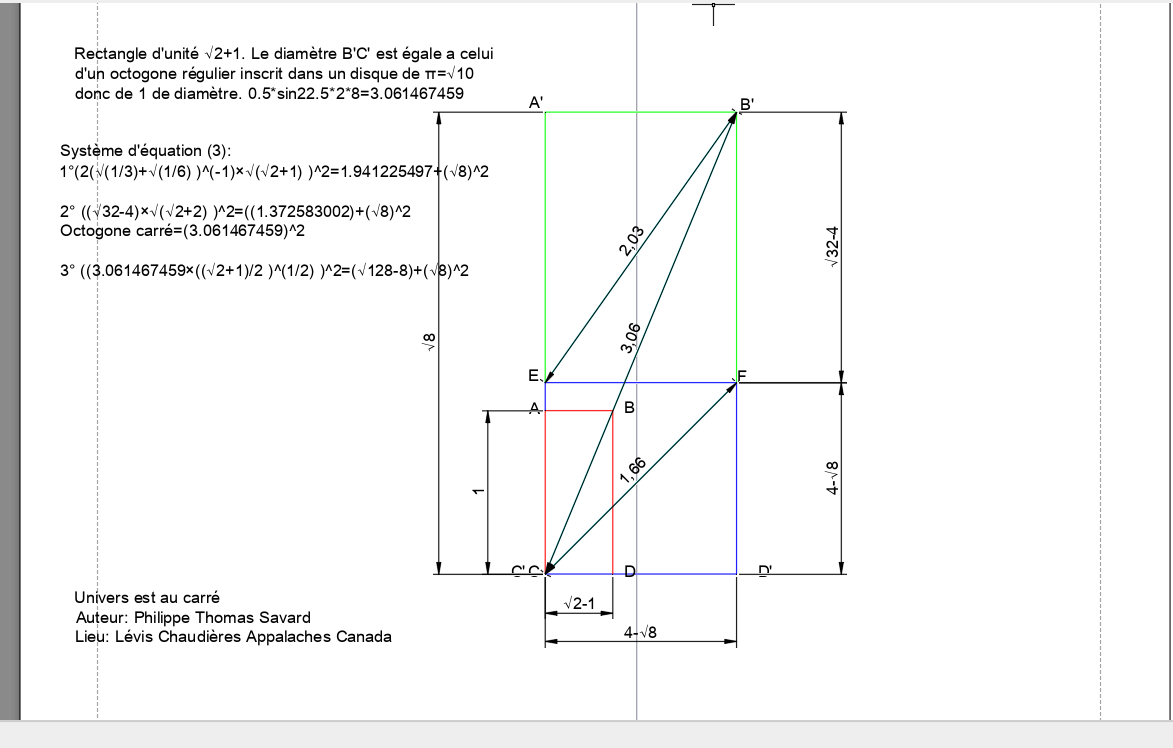
\includegraphics[width=0.85\textwidth]{racine_carre_deux.png}
\end{figure}



% --- Début du chapitre ---
\section{Explication mathématique du postulat du squaring}

\subsection{Le rectangle initial $ABCD$}

On considère un rectangle initial $ABCD$ tel que :
\[
AB = CD = \sqrt{2} - 1,
\qquad
AD = BC = 1.
\]

Son périmètre vaut :
\[
2(\sqrt{2}-1) + 2(1) = \sqrt{8}.
\]

\subsection{Élévation au carré : le rectangle $A'B'C'D'$}

En appliquant le postulat du squaring, on élève le périmètre au carré :
\[
(\sqrt{8})^2 = 8.
\]

Le rectangle transformé $A'B'C'D'$ possède alors :
\[
A'B' = C'D' = 4 - \sqrt{8},
\qquad
A'D' = B'C' = \sqrt{8}.
\]

Vérification :
\[
2(4-\sqrt{8}) + 2\sqrt{8} = 8.
\]

\subsection{Carré maximal inscrit dans $A'B'C'D'$}

Le plus grand carré inscrit dans $A'B'C'D'$ est $A'B'EF$.

Son aire vaut :
\[
(4-\sqrt{8})^2 = 1.372583002.
\]

L’aire du rectangle complet est :
\[
(4-\sqrt{8})\sqrt{8} = \sqrt{128} - 8.
\]

Le rapport des aires vaut :
\[
\frac{\sqrt{128}-8}{1.372583002} = \sqrt{2} + 1.
\]

Cette valeur devient l’unité symbolique de la mise en situation.

\subsection{Décomposition interne du rectangle transformé}

Le rectangle $A'B'C'D'$ contient :

\[
\text{Aire}(A'B'EF) = 1.372583002,
\qquad
\text{Aire}(EFC'D') = 1.941225497,
\]
\[
\text{Aire}(A'B'C'D') = \sqrt{128} - 8.
\]

On vérifie :
\[
(\sqrt{128}-8) = 1.372583002 + 1.941225497.
\]

Les dimensions des deux sous-figures sont :
\[
EF = 4 - \sqrt{8},
\qquad
C'D' = \sqrt{32} - 4.
\]

\subsection{Les trois diagonales fondamentales}

\[
\begin{aligned}
\text{Diag}(A'B'EF) &= \sqrt{32} - 4, \\
\text{Diag}(EFC'D') &= 2\left(\sqrt{\tfrac13} + \sqrt{\tfrac16}\right)^{-1}, \\
\text{Diag}(A'B'C'D') &= 3.061467459.
\end{aligned}
\]

La diagonale $A'C'$ est la mesure exacte du périmètre d’un octogone régulier inscrit dans un disque de diamètre $1$, donc :
\[
3.061467459 = \pi.
\]

Dans notre cadre géométrique :
\[
\sqrt{10} = \pi.
\]

\subsection{Les trois équations de l’octogone carré}

\[
\boxed{
\left( 2\left(\sqrt{\tfrac13}+\sqrt{\tfrac16}\right)^{-1} \sqrt{\sqrt{2}+1} \right)^2
= 1.941225497 + (\sqrt{8})^2
}
\]

\[
\boxed{
\left( (\sqrt{32}-4)\sqrt{\sqrt{2}+2} \right)^2
= 1.372583002 + (\sqrt{8})^2
}
\]

\[
\text{\small\itshape octogone carré}
\]

\[
\boxed{
\left( 3.061467459 \sqrt{\frac{\sqrt{2}+1}{2}} \right)^2
= (\sqrt{128}-8) + (\sqrt{8})^2
}
\]

\section{Appendix: Isabelle/HOL Structure formalisé du script HOL isabelle du postulat de l'univers est au carré.}

\subsection*{HOL Source Code}

\begin{minted}[bgcolor=lightgray]{isabelle}
theory postulat_carre
  imports Complex_Main
begin

(* ========================================================= *)
(* Table of Contents                                         *)
(* ========================================================= *)

(* 1. Unified Squared Rectangle and Prime Postulate          *)
(*    1.1 Locale: postulat_carre                             *)
(*    1.2 Definitions                                        *)
(*        - S_S, S_F, S_C                                    *)
(*        - d_S, d_F, d_C                                    *)
(*        - unit_p                                           *)
(*        - upto_from_2, k                                   *)
(*        - postulat_eq                                      *)
(*        - ratio_height_square                              *)
(*        - ratio_trunc_square                               *)

(* 2. Rectangle carre : equivalence avec un carre            *)
(*    2.1 Locale: rectangle_carre                            *)
(*    2.2 Area definitions                                   *)
(*    2.3 Equivalence condition                              *)

(* 3. Axiomatisation du polygone au carre                    *)
(*    3.1 Locale: polygone_carre_axiomes                     *)
(*    3.2 Height ratio equation                              *)
(*    3.3 Truncation ratio equation                          *)
(*    3.4 Postulate equation                                 *)
(*    3.5 Definition of a squared polygon                    *)

(* 4. Exemple numerique pour p = 3                           *)
(*    4.1 Locale: exemple_p3                                 *)
(*    4.2 Height ratio lemma                                 *)
(*    4.3 Truncation ratio lemma                             *)
(*    4.4 Diagonal lemma                                     *)
(*    4.5 Area lemma                                         *)

(* 5. Appendix: Full Isabelle/HOL Source Code                *)
(*    - postulat_carre.thy                                   *)

(* 6. License                                                *)

section "Unified Squared Rectangle and Prime Postulate"

locale postulat_carre =
  fixes w :: real
    and h :: real
    and s :: real
    and t :: real
    and p :: nat
    and diag :: real
    and area :: real
  assumes geom: "w > 0" "h > 0" "s > 0" "t > 0" "s <= w" "s <= h"
    and prime_p: "prime p"
begin

definition S_S :: real where
  "S_S = w * h"

definition S_F :: real where
  "S_F = s * s"

definition S_C :: real where
  "S_C = S_S - S_F"

definition d_S :: real where
  "d_S = sqrt (w * w + h * h)"

definition d_F :: real where
  "d_F = sqrt 2 * s"

definition d_C :: real where
  "d_C = sqrt (s * s + t * t)"

definition unit_p :: real where
  "unit_p = sqrt (real p) + 1"

definition upto_from_2 :: "nat list" where
  "upto_from_2 = [2 ..< Suc p]"

definition k :: nat where
  "k =
     (THE i. i < length upto_from_2
           & upto_from_2 ! i = p) + 1"

definition postulat_eq :: bool where
  "postulat_eq =
     ((diag * sqrt unit_p) ^ 2 = real k * area + h * h)"

definition ratio_height_square :: bool where
  "ratio_height_square =
     (h / s = sqrt (real p) + 1)"

definition ratio_trunc_square :: bool where
  "ratio_trunc_square =
     (t / s = sqrt (real p))"

end


section "Rectangle carre : equivalence avec un carre"

locale rectangle_carre =
  fixes w :: real
    and h :: real
    and s :: real
  assumes geom: "w > 0" "h > 0" "s > 0"
begin

definition area_rect :: real where
  "area_rect = w * h"

definition area_square :: real where
  "area_square = s * s"

definition rect_equiv_square :: bool where
  "rect_equiv_square =
     (area_rect = area_square)"

end


section "Axiomatisation du polygone au carre"

locale polygone_carre_axiomes =
  fixes p :: nat
    and h :: real
    and s :: real
    and t :: real
    and diag :: real
    and area :: real
  assumes prime_p: "prime p"
    and geom: "h > 0" "s > 0" "t > 0"
begin

definition eq_ratio_height :: bool where
  "eq_ratio_height =
     (h / s = sqrt (real p) + 1)"

definition eq_ratio_trunc :: bool where
  "eq_ratio_trunc =
     (t / s = sqrt (real p))"

definition eq_postulat :: bool where
  "eq_postulat =
     ((diag * sqrt (sqrt (real p) + 1)) ^ 2
        = area + h * h)"

definition polygone_defini :: bool where
  "polygone_defini =
     (eq_ratio_height & eq_ratio_trunc & eq_postulat)"

end
section "Exemple numerique pour p = 3"

locale exemple_p3 =
  fixes s3 :: real
    and h3 :: real
    and t3 :: real
    and diag3 :: real
    and area3 :: real
  assumes s3_pos: "s3 > 0"
    and ratio_height_3: "h3 / s3 = sqrt 3 + 1"
    and ratio_trunc_3: "t3 / s3 = sqrt 3"
    and diag_trunc_3: "sqrt (s3 * s3 + t3 * t3) = sqrt 6"
    and area_def_3: "area3 = s3 * h3"
begin

text "
Cet exemple formalise le cas p = 3.
Les valeurs numeriques (0.896575..., 1.552914..., etc.)
ne sont pas utilisees directement : seules les relations exactes
sont axiomatisées.
"

lemma hauteur_sur_cote:
  shows "h3 / s3 = sqrt 3 + 1"
  using ratio_height_3 .

lemma tronque_sur_cote:
  shows "t3 / s3 = sqrt 3"
  using ratio_trunc_3 .

lemma diagonale_tronquee_exacte:
  shows "sqrt (s3 * s3 + t3 * t3) = sqrt 6"
  using diag_trunc_3 .

lemma aire_rectangle:
  shows "area3 = s3 * h3"
  using area_def_3 .

end
end

(* ========================================================= *)
(* Apache License 2.0                                        *)
(* ========================================================= *)

(* Apache License                                            *)
(* Version 2.0, January 2004                                *)
(* http://www.apache.org/licenses/                          *)

(* TERMS AND CONDITIONS FOR USE, REPRODUCTION, AND DISTRIBUTION *)

(* 1. Definitions.                                           *)
(* "License" shall mean the terms and conditions for use,    *)
(* reproduction, and distribution as defined by Sections 1   *)
(* through 9 of this document.                              *)

(* "Licensor" shall mean the copyright owner or entity       *)
(* authorized by the copyright owner that is granting the    *)
(* License.                                                  *)

(* "Legal Entity" shall mean the union of the acting entity  *)
(* and all other entities that control, are controlled by,   *)
(* or are under common control with that entity.             *)

(* "Source" form shall mean the preferred form for making    *)
(* modifications.                                            *)

(* "Object" form shall mean any form resulting from          *)
(* mechanical transformation or translation of a Source form.*)

(* "Work" shall mean the work of authorship made available   *)
(* under the License.                                        *)

(* "Derivative Works" shall mean any work that is based on   *)
(* the Work.                                                 *)

(* "Contribution" shall mean any work submitted to the       *)
(* Licensor.                                                 *)

(* "Contributor" shall mean the Licensor and any individual  *)
(* or Legal Entity that submits a Contribution.              *)

(* 2. Grant of Copyright License.                            *)
(* Subject to the terms of this License, each Contributor    *)
(* grants you a perpetual, worldwide, non-exclusive,         *)
(* no-charge, royalty-free, irrevocable copyright license    *)
(* to reproduce, prepare Derivative Works of, publicly       *)
(* display, publicly perform, sublicense, and distribute     *)
(* the Work and such Derivative Works in Source or Object    *)
(* form.                                                     *)

(* 3. Grant of Patent License.                               *)
(* Each Contributor grants you a perpetual, worldwide,       *)
(* non-exclusive, no-charge, royalty-free, irrevocable       *)
(* patent license to make, use, offer to sell, sell, import, *)
(* and otherwise transfer the Work.                          *)

(* 4. Redistribution.                                        *)
(* You may reproduce and distribute copies of the Work or    *)
(* Derivative Works thereof in any medium, with or without   *)
(* modifications, provided that you give proper notice and   *)
(* include a copy of this License.                           *)

(* 5. Submission of Contributions.                           *)
(* Unless explicitly stated otherwise, any Contribution      *)
(* intentionally submitted for inclusion in the Work shall   *)
(* be under the terms of this License.                       *)

(* 6. Trademarks.                                            *)
(* This License does not grant permission to use trade names,*)
(* trademarks, service marks, or product names of the        *)
(* Licensor.                                                 *)

(* 7. Disclaimer of Warranty.                                *)
(* Unless required by applicable law or agreed to in writing,*)
(* the Licensor provides the Work on an "AS IS" BASIS,       *)
(* WITHOUT WARRANTIES OR CONDITIONS OF ANY KIND.             *)

(* 8. Limitation of Liability.                               *)
(* In no event shall the Licensor be liable for any damages  *)
(* arising from the use of the Work.                         *)

(* 9. Accepting Warranty or Additional Liability.            *)
(* You may offer additional warranties or liabilities        *)
(* consistent with this License, but only on your own behalf.*)

(* END OF TERMS AND CONDITIONS                               *)
\end{minted}

\begin{figure}[h!]
\centering
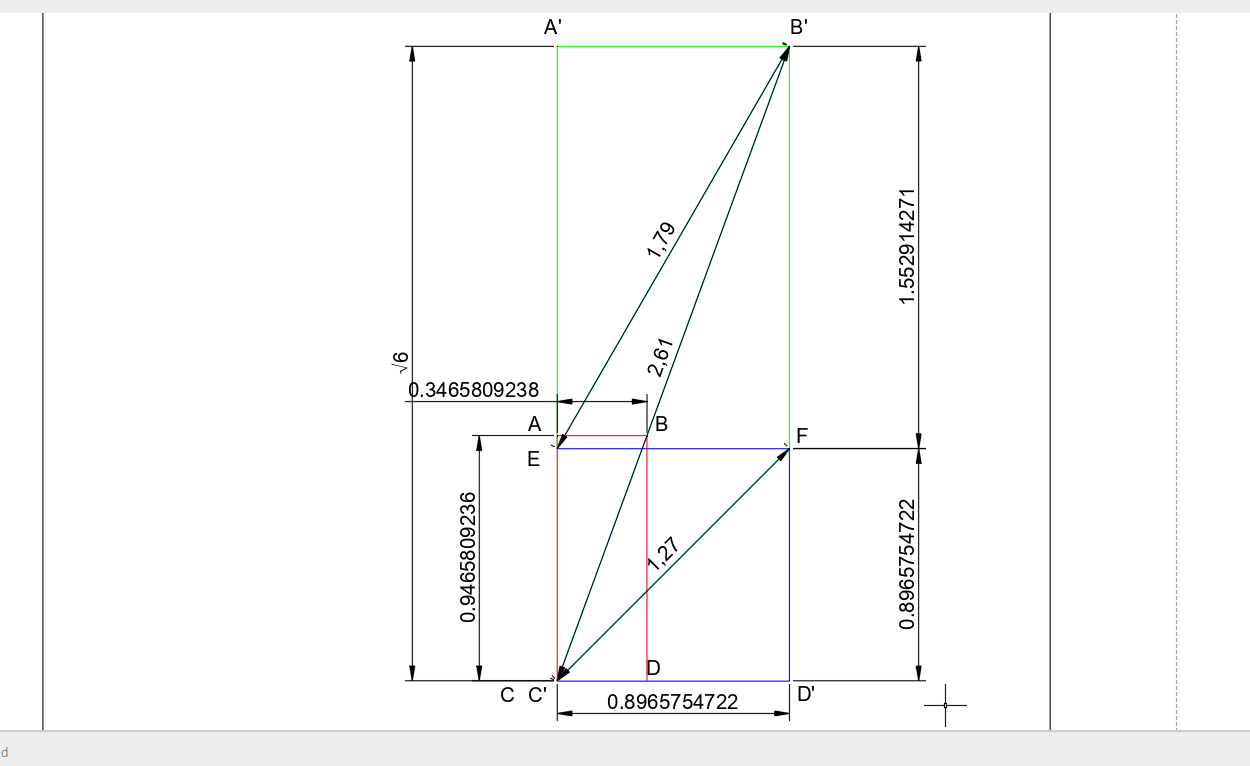
\includegraphics[width=0.85\textwidth]{racine_carre_trois.png}
\end{figure}
\setstretch{1.2}
% ---------------------------------------------------------
% SUITE DU TEXTE
% ---------------------------------------------------------

\section{Unité symbolique $\sqrt{3}+1$ : rectangle carré et hexagone carré}

\subsection*{Explication textuelle}

L’unité symbolique $\sqrt{3}+1$ donne naissance à une nouvelle famille géométrique, en parallèle à celle construite avec $\sqrt{2}+1$. Ici encore, on part d’un rectangle initial, on applique le postulat du \emph{squaring} au périmètre, puis on observe la structure interne du rectangle transformé. Cette fois, la figure mise en évidence n’est plus un octogone carré, mais un \emph{hexagone carré}.

On commence par un rectangle $ABCD$ dont les côtés sont choisis de sorte que son périmètre soit
\[
2AB + 2AD = 2.586915234.
\]
Ce périmètre est la racine carrée du périmètre d’un rectangle transformé $A'B'C'D'$, conformément au postulat du squaring. Le rectangle transformé a pour périmètre
\[
\sqrt{24} + 1.793150943 = 6.692130429.
\]
Ses côtés sont
\[
A'B' = 0.8965754715,
\qquad
A'D' = \sqrt{6},
\]
et il contient un segment horizontal $EF$ de même longueur que $A'B'$, situé à une hauteur
\[
B'F = 1.552914271.
\]

Comme dans le cas de l’unité $\sqrt{2}+1$, le rectangle transformé se décompose en deux régions : un rectangle carré $A'B'EF$ et un rectangle résiduel $EFC'D'$. Les aires et les diagonales de ces deux sous-figures, ainsi que celles du rectangle complet $A'B'C'D'$, permettent d’écrire trois équations remarquables. Ces équations mettent en relation l’unité $\sqrt{3}+1$, les longueurs internes de la figure et la diagonale du rectangle transformé.

La diagonale du rectangle transformé est liée au périmètre d’un hexagone régulier inscrit dans un disque de diamètre $1$, dont le périmètre vaut
\[
3.
\]
Ainsi, l’unité $\sqrt{3}+1$ joue pour l’hexagone un rôle analogue à celui que joue $\sqrt{2}+1$ pour l’octogone : elle encode une transformation géométrique où rectangle, carré et hexagone se répondent dans une même structure de squaring.

\subsection*{Développement en calculs}

\paragraph{Rectangle initial $ABCD$.}

On considère un rectangle initial $ABCD$ tel que :
\[
AB = 0.3465809239,
\qquad
AD = 0.9468766931.
\]
Son périmètre vaut :
\[
2(0.3465809239) + 2(0.9468766931)
= 2.586915234.
\]

\subsection{Rectangle transformé}

En appliquant le postulat du squaring, le périmètre du rectangle transformé est :
\[
\sqrt{24} + 1.793150943 = 6.692130429.
\]

Le rectangle $A'B'C'D'$ possède :
\[
A'B' = 0.8965754715, \qquad
A'D' = \sqrt{6}, \qquad
EF = 0.8965754715, \qquad
B'F = 1.552914271.
\]

\[
\boxed{
\left( 1.793150943 \,\sqrt{\sqrt{3}+1} \right)^2
= 2(0.8965754715 \times 1.552914271) + (\sqrt{6})^2
}
\]

\[
\boxed{
\left( (3-\sqrt{3})\sqrt{\sqrt{3}+3} \right)^2
= 2(0.8038475761) + (\sqrt{6})^2
}
\]

\[
\text{\small\itshape hexagone carré}
\]

\[
\boxed{
\left( 2.608418597 \,\sqrt{\frac{2}{4-\sqrt{3}}\,\sqrt{3}} \right)^2
= 2(0.8965754715 \times \sqrt{6}) + (\sqrt{6})^2
}
\]

Enfin, le périmètre de l’hexagone régulier inscrit dans un disque de diamètre $1$ vaut :
\[
0.5 \times \sin(30^\circ) \times 2 \times 6 = 3.
\]

Ces trois équations définissent la figure élevée au carré associée à l’unité $\sqrt{3}+1$ :
\[
\text{l’hexagone carré}.
\]

\begin{figure}[h!]
    \centering
    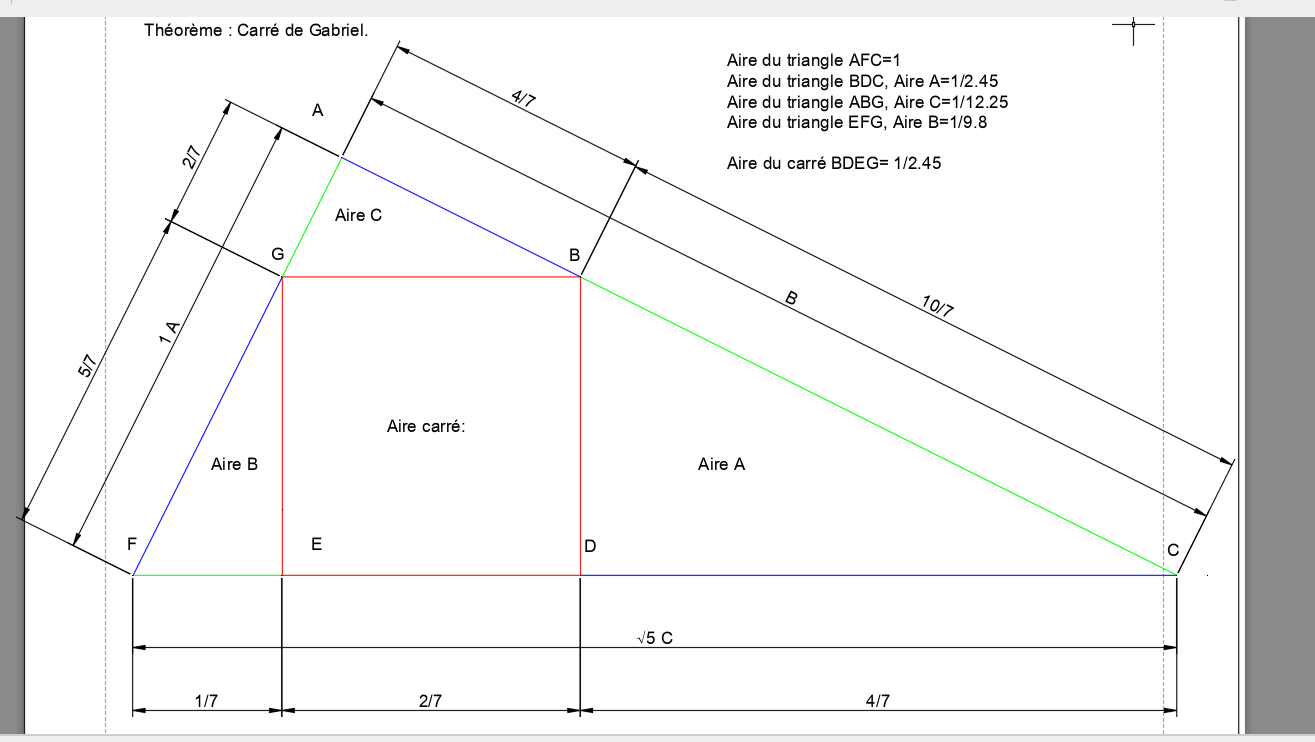
\includegraphics[width=0.85\textwidth]{triangle_carre_gabriel.png}
    \caption{Triangle rectangle AFC et carré inscrit — Théorème du carré de Gabriel}
    \label{fig:triangle_carre_gabriel}
\end{figure}

\section*{Résumé de la méthode}

La méthode du carré de Gabriel repose sur l’idée qu’un triangle peut être entièrement décrit à partir du plus grand carré que l’on peut inscrire en son intérieur. Ce carré divise le triangle complet en trois triangles secondaires dont les aires sont directement liées aux côtés du triangle d’origine.

Le principe fondamental est que le carré d’un côté du triangle complet, multiplié par l’aire du triangle opposé et divisé par l’aire du carré inscrit, donne toujours l’aire totale du triangle. Cette relation est vraie pour chacun des trois côtés, ce qui permet de vérifier la cohérence géométrique du triangle et de retrouver son aire totale.

Une seconde version de la méthode utilise le cube des côtés plutôt que leur carré. Dans ce cas, la même relation permet de retrouver la longueur des côtés du triangle complet. Ainsi, les aires des triangles secondaires et l’aire du carré inscrit suffisent pour reconstruire toute la géométrie du triangle.

La méthode s’applique aussi bien aux triangles rectangles qu’aux triangles scalènes. Dans tous les cas, les rapports obtenus révèlent des constantes internes remarquables, montrant que le carré inscrit agit comme un invariant géométrique reliant les aires et les longueurs du triangle.

\subsection*{Théorème de Gabriel — Triangle rectangle}

\begin{itemize}
    \item Aire totale du triangle AFC : $1$
    \item Aire du triangle BDC (Aire A) : $1/2.45$
    \item Aire du triangle ABG (Aire C) : $1/12.25$
    \item Aire du triangle EFG (Aire A) : $1/9.8$
    \item Aire du carré BDEG : $1/2.45$
\end{itemize}

Les équations fondamentales :
\[
\frac{1^2 \times (1/2.45)}{1/2.45} = 1
\]
\[
\frac{2^2 \times (1/9.8)}{1/2.45} = 1
\]
\[
\frac{(\sqrt{5})^2 \times (1/12.25)}{1/2.45} = 1
\]

Version pour retrouver les longueurs :
\[
\frac{1^3 \times (1/2.45)}{1/2.45} = 1
\]
\[
\frac{2^3 \times (1/9.8)}{1/2.45} = 2
\]
\[
\frac{(\sqrt{5})^3 \times (1/12.25)}{1/2.45} = \sqrt{5}
\]

\begin{figure}[h!]
    \centering
    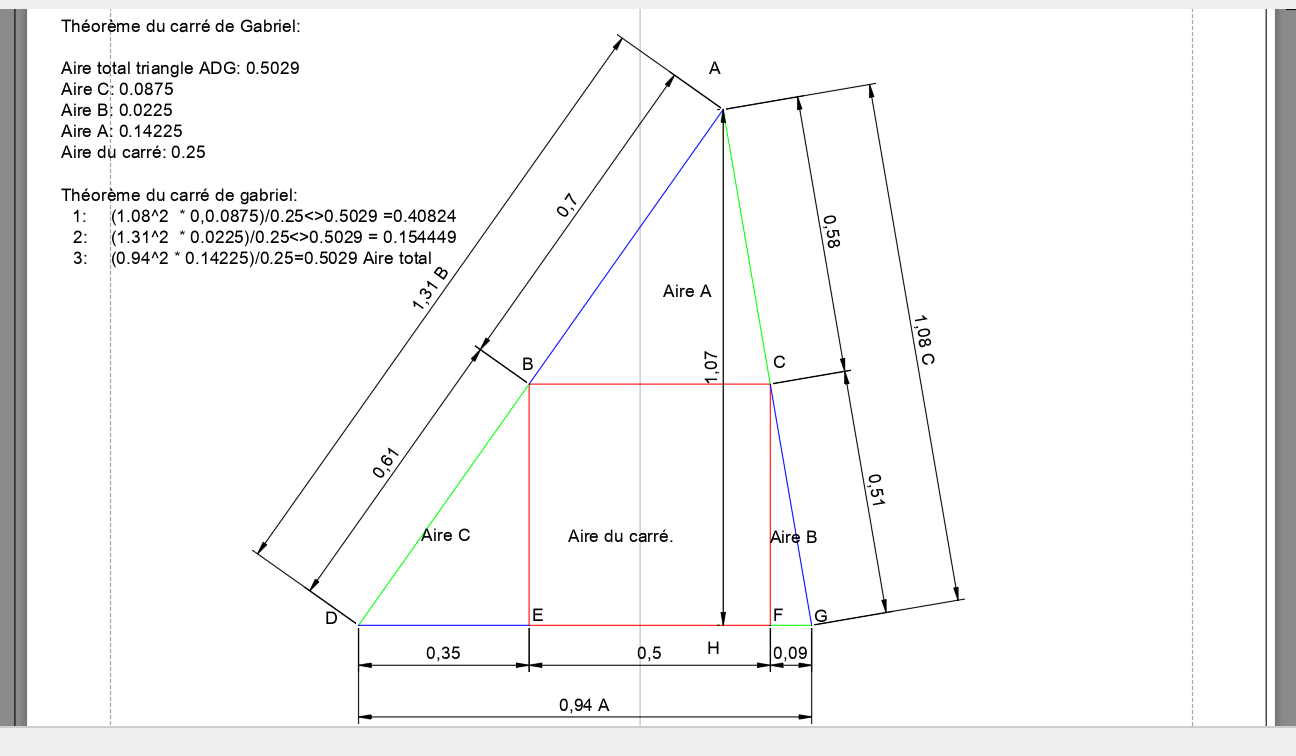
\includegraphics[width=0.85\textwidth]{triangle_carre_gabriel_scalene.png}
    \caption{Triangle scalène ADG et carré inscrit — Version généralisée du théorème de Gabriel}
    \label{fig:triangle_carre_gabriel_scalene}
\end{figure}

\subsection*{Théorème de Gabriel — Triangle scalène}

Aire du triangle complet :
\[
(0.9393398282 \times 1.06935594)/2 = 0.5020938555
\]

Aires secondaires :
\[
A_C = \sqrt{1/128}, \qquad
A_B = 0.0214466094, \qquad
A_A = 0.1422588985
\]

Équations :
\[
\frac{1.084656205^2 \times \sqrt{1/128}}{0.25} = 0.4159481688
\]
\[
\frac{1.309295861^2 \times 0.0214466094}{0.25} = 0.1470598855
\]
\[
\frac{0.9393398282^2 \times 0.1422588985}{0.25} = 0.5020938555
\]

Rapports remarquables :
\[
\frac{0.5020938555}{0.4159481688} = \frac{\sqrt{2}+1}{2}
\]
\[
\frac{0.5020938555}{0.1470598855} = \sqrt{2}+2
\]

\end{document}